\section{Model Test}
%===================

This section details the forward/tangent-linear and tangent-linear/adjoint tests performed on the main subroutines: \texttt{LowFrequency\_MWSSEM()}, \texttt{LowFrequency\_MWSSEM\_TL()}, and \texttt{LowFrequency\_MWSSEM\_AD()}. The number of input test values and their ranges of the input forward variables are shown in table \ref{tab:main_input_range}. The actual values used are evenly distributed between the minimum and maximum, inclusively. 
\begin{table}[htp]
  \centering
  \begin{tabular}{| c | c | r@{.}l@{ - }r@{.}l | c |}
    \hline
    \textbf{Quantity} & \textbf{\# of Values} & \multicolumn{4}{c|}{\textbf{Range}} & \textbf{Units} \\
    \hline\hline
    Frequency    & 16 &   5&0 &  20&0 & GHz \\
    Zenith angle &  7 &   0&0 &  60&0 & Deg. \\
    Temperature  & 11 & 273&0 & 303&0 & K \\
    Salinity     &  5 &  20&0 &  40&0 & \textperthousand \\
    Wind speed   & 21 &   2&0 &  19&0 & m.s$^{-1}$ \\
    \hline
  \end{tabular}
  \caption{Range of test input data to main LF MWSSEM routines}
  \label{tab:main_input_range}
\end{table}
The number of frequency and wind speed values were chosen such that there was not always correspondence with the hinge points of the ocean height variance lookup table (LUT). This ensures that the interpolation of the LUT data is included in the testing.

Forward model results for two test frequencies (7.0GHz and 19.0GHz)\footnote{AMSR-E channel 1 and 3 frequencies are 6.925GHz and  18.7GHz respectively.}, one zenith angle (30$^\circ$), and one salinity value (35\textperthousand) are shown in figure \ref{fig:fwd_emissivity}. As mentioned in section \ref{sec:model_description}, for wind speeds greater than 7.0ms$^{-1}$ the Fresnel reflectivities are modified to account for surface foam and this shows up in the forward results as a discontinuity between 7.0 and 8.0ms$^{-1}$ (most evident in figure \ref{fig:fwd_emissivity}(b)). 
\begin{figure}[htp]
  \centering
  \begin{tabular}{c c}
    \multicolumn{2}{c}{\sffamily\textbf{\textbfm{f}=7.0GHz, \textbfm{\theta_i}=30$^\circ$, S=35\textperthousand}}\\
    \textsf{(a) Vertical Polarisation} &
    \textsf{(b) Horizontal Polarization} \\
    \includegraphics[bb=110 240 508 540,clip,scale=0.5]{graphics/Model/ev_s35.0ppt_z30.0_7.00GHz.eps} &
    \includegraphics[bb=110 240 508 540,clip,scale=0.5]{graphics/Model/eh_s35.0ppt_z30.0_7.00GHz.eps} \\\\

    \multicolumn{2}{c}{\sffamily\textbf{\textbfm{f}=19.0GHz, \textbfm{\theta_i}=30$^\circ$, S=35\textperthousand}}\\
    \textsf{(c) Vertical Polarisation} &
    \textsf{(d) Horizontal Polarization} \\
    \includegraphics[bb=110 240 508 540,clip,scale=0.5]{graphics/Model/ev_s35.0ppt_z30.0_19.00GHz.eps} &
    \includegraphics[bb=110 240 508 540,clip,scale=0.5]{graphics/Model/eh_s35.0ppt_z30.0_19.00GHz.eps}
  \end{tabular}
  \caption{Computed vertical and horizontal polarised emissivities at two frequencies $<$ 20GHz, a zenith angle of 30$^\circ$, a salinity of 35\textperthousand, and for a range of ocean surface wind speeds and temperatures. The feature seen at 7m.s$^{-1}$ is due to the modification of the reflectivity due to foam cover.}
  \label{fig:fwd_emissivity}
\end{figure}


\subsection{FWD/TL Test Results}
%-------------------------------
The description of the FWD/TL tests for routines with real valued output is given in section \ref{sec:fwdtl_test}. Some representative results are shown in figure \ref{fig:fwdtl_a0.1000_7.00GHz_emissivity} for 7.0GHz and an alpha value of 0.1. The aforementioned discontinuity seen at wind speeds of 7.0ms$^{-1}$ is quite evident in the non-linear and tangent-linear responses (figures \ref{fig:fwdtl_a0.1000_7.00GHz_emissivity}(a)-(d)). The relatively large value of alpha means the perturbation is also relatively large and as such, the test residuals of figures \ref{fig:fwdtl_a0.1000_7.00GHz_emissivity}(e) and (f) still exhibit some functional characteristics. When the value of alpha is decreased to 0.0001, while the responses themselves appear similar, the test residuals decrease to the point where it appears calculation ``noise'' predominates, as shown in figure \ref{fig:fwdtl_a0.0001_7.00GHz_emissivity}. This is expected as the perturbation applied is much smaller and thus the forward model response is correspondingly more linear. The maximum tolerance residual for each value of alpha is shown in table \ref{tab:fwdtl_alpha}. As expected, as alpha decreases so do the tolerance residuals since.
\begin{table}[htp]
  \centering
  \begin{tabular}{| c | c |}
    \hline
    \boldmath$\alpha$\unboldmath & \textbf{Tolerance residual,} \boldmath$t_r$\unboldmath \\
    \hline\hline
    0.1    & 2.0e-06 \\
    0.01   & 2.0e-07 \\
    0.001  & 2.0e-08 \\
    0.0001 & 2.0e-09 \\
    \hline
  \end{tabular}
  \caption{Maximum tolerance residuals for the emissivity FWD/TL tests.}
  \label{tab:fwdtl_alpha}
\end{table}

Test results for an alpha value of 0.1 but for a frequency of 19.0GHz are shown in figure \ref{fig:fwdtl_a0.1000_19.00GHz_emissivity}. The character of the non-linear and tangent-linear responses is very different to that seen for the 7.0GHz case. The unevenness seen along the wind speed dimension is due to the small scale correction applied for frequencies greater than 15GHz. Smaller residuals, but with the same characteristics spikes, were seen for the  19.0GHz case but with an alpha value of 0.0001, as shown in figure \ref{fig:fwdtl_a0.0001_19.00GHz_emissivity}.

As described in section \ref{sec:small_scale_correction}, the ocean height variance is used in the small-scale reflectivity correction. Figure \ref{fig:sdd_wind_speed_spectra}(a) shows the ocean height variance as a function of wind speed for various frequencies. Although they appear relatively smmoth, removal of the mean slope, as shown in figure \ref{fig:sdd_wind_speed_spectra}(b), shows how noisy the data is, which translates to the perturbation surfaces of figure \ref{fig:fwdtl_a0.1000_19.00GHz_emissivity}. Additionally, the large spikes in the test residuals of figures \ref{fig:fwdtl_a0.1000_19.00GHz_emissivity}(e) and (f) occur at wind speeds of 2.0, 10.5, and 19.0ms$^{-1}$ which are all hingepoints in the ocean height variance LUT.

To determine if the noisy height displacement data is the cause of these wind speed hingepoint spikes, the data was smoothed using a Savitsky-Golay filter (see chapter 14 of \citet{NumericalRecipes_Fortran}) of width 6ms$^{-1}$ and 40GHz in the wind speed and frequency dimensions respectively. The smoothed height variance mean difference wind speed spectra are shown in figure \ref{fig:sddsmthd_wind_speed_spectra}. The FWD/TL residuals using this smoothed data are shown in figure \ref{fig:smthdfwdtl_a0.0001_19.00GHz_emissivity} where they are approximately 2-10 times less than those using the original data, but still exhibit the anomalous peaks at the wind speed hingepoints.

Repeating the tests for different wind speed grids such that interpolation was performed primarily between, and not across, hingepoints led to the residuals shown in figure \ref{fig:fwdtl_wtest_a0.0001_19.00GHz_emissivity}. Only the vertically polarised results are shown. Two tests were run: one where the edge value wind speeds were selected to not coincide with a LUT hingepoint but an intermediate value of 10.5ms$^{-1}$ did, as seen in figure \ref{fig:fwdtl_wtest_a0.0001_19.00GHz_emissivity}(a); and one where there were no test wind speed values near LUT hingepoints, as seen in figure \ref{fig:fwdtl_wtest_a0.0001_19.00GHz_emissivity}(b). It appears that the forward model is particularly sensitive to perturbations about the LUT wind speed hingepoints, even when using the smoothed data.

Because perturbations along the temperature dimension do not exhibit the same behaviour, it suggests the integrations done on the ocean wave spectra of \citet{BjerkaasRiedel_1979} to derive the various height variance values, $\zeta^2_R$, should be recomputed. Since the residuals are of the order of 0.05\% it may be unnecessary, but it does make objective validation of the tangent-linear model difficult.

\begin{figure}[htp]
  \centering
  \begin{tabular}{c c}
    \multicolumn{2}{c}{\sffamily\textbf{Non-linear difference}}\\
    \textsf{(a)} $\Delta e_v$ &
    \textsf{(b)} $\Delta e_h$ \\
    \includegraphics[bb=110 240 508 540,clip,scale=0.5]{graphics/Model/FWDTL/Initial/FWDdev_a0.1000_s35.0ppt_z30.0_7.00GHz.eps} &
    \includegraphics[bb=110 240 508 540,clip,scale=0.5]{graphics/Model/FWDTL/Initial/FWDdeh_a0.1000_s35.0ppt_z30.0_7.00GHz.eps} \\\\
    \multicolumn{2}{c}{\sffamily\textbf{Tangent-linear response}}\\
    \textsf{(c)} $\delta e_v$ &
    \textsf{(d)} $\delta e_h$ \\
    \includegraphics[bb=110 240 508 540,clip,scale=0.5]{graphics/Model/FWDTL/Initial/TLdev_a0.1000_s35.0ppt_z30.0_7.00GHz.eps} &
    \includegraphics[bb=110 240 508 540,clip,scale=0.5]{graphics/Model/FWDTL/Initial/TLdeh_a0.1000_s35.0ppt_z30.0_7.00GHz.eps} \\\\
    \multicolumn{2}{c}{\sffamily\textbf{Forward/tangent-linear test result}}\\
    \textsf{(e)} $|\Delta e_v - \delta e_v|$ &
    \textsf{(f)} $|\Delta e_h - \delta e_h|$ \\
    \includegraphics[bb=110 240 508 540,clip,scale=0.5]{graphics/Model/FWDTL/Initial/FWDTLtestev_a0.1000_s35.0ppt_z30.0_7.00GHz.eps} & 
    \includegraphics[bb=110 240 508 540,clip,scale=0.5]{graphics/Model/FWDTL/Initial/FWDTLtesteh_a0.1000_s35.0ppt_z30.0_7.00GHz.eps}
  \end{tabular}
  \caption{Computed emissivities at 7GHz for the forward/tangent-linear test with $\alpha$=0.1. \textbf{(a)} Vertically polarised non-linear difference.  \textbf{(b)} Horizontally polarised non-linear difference. \textbf{(c)} Vertically polarised tangent-linear response. \textbf{(d)} Horizontally polarised tangent-linear response. \textbf{(e)} Vertically polarised test residual. \textbf{(f)} Horizontally polarised test residual.}
  \label{fig:fwdtl_a0.1000_7.00GHz_emissivity}
\end{figure}

\begin{figure}[htp]
  \centering
  \begin{tabular}{c c}
    \multicolumn{2}{c}{\sffamily\textbf{Forward/tangent-linear test result}}\\
    \textsf{(a)} $|\Delta e_v - \delta e_v|$ &
    \textsf{(b)} $|\Delta e_h - \delta e_h|$ \\
    \includegraphics[bb=110 240 508 540,clip,scale=0.5]{graphics/Model/FWDTL/Initial/FWDTLtestev_a0.0001_s35.0ppt_z30.0_7.00GHz.eps} & 
    \includegraphics[bb=110 240 508 540,clip,scale=0.5]{graphics/Model/FWDTL/Initial/FWDTLtesteh_a0.0001_s35.0ppt_z30.0_7.00GHz.eps}
  \end{tabular}
  \caption{Forward/tangent-linear test residuals at 7GHz for $\alpha$=0.0001. \textbf{(a)} Vertically polarised test residual (compare with figure \ref{fig:fwdtl_a0.1000_7.00GHz_emissivity}(e)). \textbf{(b)} Horizontally polarised test residual (compare with figure \ref{fig:fwdtl_a0.1000_7.00GHz_emissivity}(f)).}
  \label{fig:fwdtl_a0.0001_7.00GHz_emissivity}
\end{figure}

\begin{figure}[htp]
  \centering
  \begin{tabular}{c c}
    \multicolumn{2}{c}{\sffamily\textbf{Non-linear difference}}\\
    \textsf{(a)} $\Delta e_v$ &
    \textsf{(b)} $\Delta e_h$ \\
    \includegraphics[bb=110 240 508 540,clip,scale=0.5]{graphics/Model/FWDTL/Initial/FWDdev_a0.1000_s35.0ppt_z30.0_19.00GHz.eps} &
    \includegraphics[bb=110 240 508 540,clip,scale=0.5]{graphics/Model/FWDTL/Initial/FWDdeh_a0.1000_s35.0ppt_z30.0_19.00GHz.eps} \\\\
    \multicolumn{2}{c}{\sffamily\textbf{Tangent-linear response}}\\
    \textsf{(c)} $\delta e_v$ &
    \textsf{(d)} $\delta e_h$ \\
    \includegraphics[bb=110 240 508 540,clip,scale=0.5]{graphics/Model/FWDTL/Initial/TLdev_a0.1000_s35.0ppt_z30.0_19.00GHz.eps} &
    \includegraphics[bb=110 240 508 540,clip,scale=0.5]{graphics/Model/FWDTL/Initial/TLdeh_a0.1000_s35.0ppt_z30.0_19.00GHz.eps} \\\\
    \multicolumn{2}{c}{\sffamily\textbf{Forward/tangent-linear test result}}\\
    \textsf{(e)} $|\Delta e_v - \delta e_v|$ &
    \textsf{(f)} $|\Delta e_h - \delta e_h|$ \\
    \includegraphics[bb=110 240 508 540,clip,scale=0.5]{graphics/Model/FWDTL/Initial/FWDTLtestev_a0.1000_s35.0ppt_z30.0_19.00GHz.eps} & 
    \includegraphics[bb=110 240 508 540,clip,scale=0.5]{graphics/Model/FWDTL/Initial/FWDTLtesteh_a0.1000_s35.0ppt_z30.0_19.00GHz.eps}
  \end{tabular}
  \caption{Computed emissivities at 19GHz for the forward/tangent-linear test with $\alpha$=0.1. \textbf{(a)} Vertically polarised non-linear difference.  \textbf{(b)} Horizontally polarised non-linear difference. \textbf{(c)} Vertically polarised tangent-linear response. \textbf{(d)} Horizontally polarised tangent-linear response. \textbf{(e)} Vertically polarised test residual. \textbf{(f)} Horizontally polarised test residual.}
  \label{fig:fwdtl_a0.1000_19.00GHz_emissivity}
\end{figure}

\begin{figure}[htp]
  \centering
  \begin{tabular}{c c}
    \multicolumn{2}{c}{\sffamily\textbf{Forward/tangent-linear test result}}\\
    \textsf{(a)} $|\Delta e_v - \delta e_v|$ &
    \textsf{(b)} $|\Delta e_h - \delta e_h|$ \\
    \includegraphics[bb=110 240 508 540,clip,scale=0.5]{graphics/Model/FWDTL/Initial/FWDTLtestev_a0.0001_s35.0ppt_z30.0_19.00GHz.eps} & 
    \includegraphics[bb=110 240 508 540,clip,scale=0.5]{graphics/Model/FWDTL/Initial/FWDTLtesteh_a0.0001_s35.0ppt_z30.0_19.00GHz.eps}
  \end{tabular}
  \caption{Forward/tangent-linear test residuals at 19GHz for $\alpha$=0.0001. \textbf{(a)} Vertically polarised test residual (compare with figure \ref{fig:fwdtl_a0.1000_19.00GHz_emissivity}(e)). \textbf{(b)} Horizontally polarised test residual (compare with figure \ref{fig:fwdtl_a0.1000_19.00GHz_emissivity}(f)).}
  \label{fig:fwdtl_a0.0001_19.00GHz_emissivity}
\end{figure}

\begin{figure}[htp]
  \centering
  \begin{tabular}{c}
    \textsf{(a) Ocean height variance $(4k^2\zeta^2_R)$ wind speed spectra}\\
    \includegraphics[bb=85 400 540 560,clip,scale=0.9]{graphics/LUT/sdd_wind_speed_spectra.eps}\\
    \textsf{(b) Ocean height variance $(4k^2\zeta^2_R)$ mean difference wind speed spectra}\\
    \includegraphics[bb=85 225 540 384,clip,scale=0.9]{graphics/LUT/sdd_wind_speed_spectra.eps}
  \end{tabular}
  \caption{Ocean height variance wind speed spectra used for the small-scale reflectivity correction. \textbf{(a)} Actual height variance spectra in the LUT. Dashed black line is the linear fit to the average for all frequencies. \textbf{(b)} Height variance mean difference spectra obtained by subtracted the mean value and slope from the data, highlighting the noisiness in the LUT data.}
  \label{fig:sdd_wind_speed_spectra}
\end{figure}

\begin{figure}[htp]
  \centering
  \includegraphics[bb=85 225 540 384,clip,scale=0.9]{graphics/LUT/sddsmthd_wind_speed_spectra.eps}
  \caption{Ocean height variance mean difference spectra obtained from smoothed data. Original data was smoothed using a Savitzky-Golay filter in both the wind speed and frequency dimensions. Compare with figure \ref{fig:sdd_wind_speed_spectra}(b).}
  \label{fig:sddsmthd_wind_speed_spectra}
\end{figure}

\begin{figure}[htp]
  \centering
  \begin{tabular}{c c}
    \multicolumn{2}{c}{\sffamily\textbf{Forward/tangent-linear test result}}\\
    \textsf{(a)} $|\Delta e_v - \delta e_v|$ &
    \textsf{(b)} $|\Delta e_h - \delta e_h|$ \\
    \includegraphics[bb=110 240 508 540,clip,scale=0.5]{graphics/Model/FWDTL/Smoothed/FWDTLtestev_a0.1000_s35.0ppt_z30.0_19.00GHz.eps} & 
    \includegraphics[bb=110 240 508 540,clip,scale=0.5]{graphics/Model/FWDTL/Smoothed/FWDTLtesteh_a0.1000_s35.0ppt_z30.0_19.00GHz.eps}
  \end{tabular}
  \caption{Forward/tangent-linear test residuals at 19GHz for $\alpha$=0.1 using the smoothed ocean height variance spectra. Peak residuals are $\sim$2-10 times less than those using the original height variance data. \textbf{(a)} Vertically polarised test residual (compare with figure \ref{fig:fwdtl_a0.1000_19.00GHz_emissivity}(e)). \textbf{(b)} Horizontally polarised test residual (compare with figure \ref{fig:fwdtl_a0.1000_19.00GHz_emissivity}(f)).}
  \label{fig:smthdfwdtl_a0.0001_19.00GHz_emissivity}
\end{figure}

\begin{figure}[htp]
  \centering
  \begin{tabular}{c c}
    \multicolumn{2}{c}{\sffamily\textbf{Forward/tangent-linear test result}}\\
    \textsf{(a) Wind speed test gridpoint at} &
    \textsf{(b) No wind speed test gridpoint}  \\
    \textsf{LUT hingepoint of 10ms\textbfm{^{\textsf{-1}}}} &
    \textsf{corresponds with LUT hingepoints}  \\
    \includegraphics[bb=110 240 508 540,clip,scale=0.5]{graphics/Model/FWDTL/Initial/FWDTLtestev_wtest1_a0.0001_s35.0ppt_z30.0_19.00GHz.eps} & 
    \includegraphics[bb=110 240 508 540,clip,scale=0.5]{graphics/Model/FWDTL/Initial/FWDTLtestev_wtest2_a0.0001_s35.0ppt_z30.0_19.00GHz.eps}
  \end{tabular}
  \caption{Forward/tangent-linear vertically polarised test residuals at 19GHz for $\alpha$=0.0001 for different wind speed grid spacings. Compare with figure \ref{fig:fwdtl_a0.0001_19.00GHz_emissivity}(a). \textbf{(a)} Edge wind speed values no longer correspond with LUT hingepoints, but centre value at 10ms\textbfm{^{\textsf{-1}}} does . \textbf{(b)} No wind speed values correspond with LUT hingepoints.}
  \label{fig:fwdtl_wtest_a0.0001_19.00GHz_emissivity}
\end{figure}


\subsection{TL/AD Test Results}
%------------------------------
Following the description of the TL/AD test in section \ref{sec:tlad_test} for routines with both real valued input and output, the TL/AD test performed for the model was,
\begin{equation}
  \underbrace{\left[\delta e_v^2 + \delta e_h^2\right]}_{\mathbf{TL}^{T}\mathbf{TL}} - \underbrace{\left[\delta{T}.\dstar T + \delta{S}.\dstar S + \delta{W}.\dstar W\right]}_{\mathbf{\delta x}^{T}\mathbf{AD}(TL)} = 0
  \label{eqn:tlad_model}
\end{equation}
where T, S, and W are the sea surface temperature, salinity, and surface wind speed respectively (TL inputs are set to 0.1 in all cases); and $e_v$ and $e_h$ are the vertically and horizontally polarised sea surface emissivities. Examples of the intermediate quanitites and test residual used in this test are shown in figure \ref{fig:tlad_s35.0ppt_z30.0_7.00GHz} for $f$ = 7.0GHz and figure \ref{fig:tlad_s35.0ppt_z30.0_19.00GHz} for  $f$ = 19.0GHz, both for salinities of 35\textperthousand. In both cases, the residual differences are within numerical preicsion. Additionally, these results are typical for other frequencies and salinities tested.

\begin{figure}[htp]
  \centering
  \begin{tabular}{c c}
    \multicolumn{2}{c}{\sffamily\textbf{Tangent-linear emissivities}}\\
    \textsf{(a)} $\delta r_v$ &
    \textsf{(b)} $\delta r_h$ \\
    \includegraphics[bb=120 240 508 540,clip,scale=0.5]{graphics/Model/TLAD/ev_TL_s35.0ppt_z30.0_7.00GHz.eps} &
    \includegraphics[bb=120 240 508 540,clip,scale=0.5]{graphics/Model/TLAD/eh_TL_s35.0ppt_z30.0_7.00GHz.eps} \\\\
    \multicolumn{2}{c}{\sffamily\textbf{Adjoint temperature and salinity}}\\
    \textsf{(c)} $\dstar T$ &
    \textsf{(d)} $\dstar S$ \\
    \includegraphics[bb=115 240 508 540,clip,scale=0.5]{graphics/Model/TLAD/t_AD_s35.0ppt_z30.0_7.00GHz.eps} &
    \includegraphics[bb=110 240 508 540,clip,scale=0.5]{graphics/Model/TLAD/s_AD_s35.0ppt_z30.0_7.00GHz.eps} \\\\
    {\sffamily\textbf{Adjoint wind speed}} & {\sffamily\textbf{Test residual}} \\
    \textsf{(e)} $\dstar T$ &
    \textsf{(f)} $\mathbf{TL}^{T}\mathbf{TL} - \mathbf{\delta x}^{T}\mathbf{AD}(TL)$ \\
    \includegraphics[bb=110 240 508 540,clip,scale=0.5]{graphics/Model/TLAD/w_AD_s35.0ppt_z30.0_7.00GHz.eps} & 
    \includegraphics[bb=110 240 508 540,clip,scale=0.5]{graphics/Model/TLAD/TLtTL-dxtAD_s35.0ppt_z30.0_7.00GHz.eps}
  \end{tabular}
  \caption{Example of quantities used to test the TL/AD routines for $\delta{T}$, $\delta{S}$, and $\delta{W}$ inputs of 0.1, a salinity of 35\textperthousand, an incidence angle of 30$^{\circ}$ at a frequency of 7.0GHz. \textbf{(a)} Tangent-linear vertical emissivity. \textbf{(b)} Tangent-linear horizontal emissivity. \textbf{(c)} Adjoint temperature.  \textbf{(d)} Adjoint salinity. \textbf{(e)} Adjoint wind speed. \textbf{(f)} Test residual (see eqn.\ref{eqn:tlad_model}).}
  \label{fig:tlad_s35.0ppt_z30.0_7.00GHz}
\end{figure}

\begin{figure}[htp]
  \centering
  \begin{tabular}{c c}
    \multicolumn{2}{c}{\sffamily\textbf{Tangent-linear emissivities}}\\
    \textsf{(a)} $\delta r_v$ &
    \textsf{(b)} $\delta r_h$ \\
    \includegraphics[bb=120 240 508 540,clip,scale=0.5]{graphics/Model/TLAD/ev_TL_s35.0ppt_z30.0_19.00GHz.eps} &
    \includegraphics[bb=120 240 508 540,clip,scale=0.5]{graphics/Model/TLAD/eh_TL_s35.0ppt_z30.0_19.00GHz.eps} \\\\
    \multicolumn{2}{c}{\sffamily\textbf{Adjoint temperature and salinity}}\\
    \textsf{(c)} $\dstar T$ &
    \textsf{(d)} $\dstar S$ \\
    \includegraphics[bb=115 240 508 540,clip,scale=0.5]{graphics/Model/TLAD/t_AD_s35.0ppt_z30.0_19.00GHz.eps} &
    \includegraphics[bb=110 240 508 540,clip,scale=0.5]{graphics/Model/TLAD/s_AD_s35.0ppt_z30.0_19.00GHz.eps} \\\\
    {\sffamily\textbf{Adjoint wind speed}} & {\sffamily\textbf{Test residual}} \\
    \textsf{(e)} $\dstar T$ &
    \textsf{(f)} $\mathbf{TL}^{T}\mathbf{TL} - \mathbf{\delta x}^{T}\mathbf{AD}(TL)$ \\
    \includegraphics[bb=110 240 508 540,clip,scale=0.5]{graphics/Model/TLAD/w_AD_s35.0ppt_z30.0_19.00GHz.eps} & 
    \includegraphics[bb=110 240 508 540,clip,scale=0.5]{graphics/Model/TLAD/TLtTL-dxtAD_s35.0ppt_z30.0_19.00GHz.eps}
  \end{tabular}
  \caption{Example of quantities used to test the TL/AD routines for $\delta{T}$, $\delta{S}$, and $\delta{W}$ inputs of 0.1, a salinity of 35\textperthousand, an incidence angle of 30$^{\circ}$ at a frequency of 19.0GHz. \textbf{(a)} Tangent-linear vertical emissivity. \textbf{(b)} Tangent-linear horizontal emissivity. \textbf{(c)} Adjoint temperature.  \textbf{(d)} Adjoint salinity. \textbf{(e)} Adjoint wind speed. \textbf{(f)} Test residual (see eqn.\ref{eqn:tlad_model}).}
  \label{fig:tlad_s35.0ppt_z30.0_19.00GHz}
\end{figure}
